%%% File encoding: UTF-8
%% äöüÄÖÜß  <-- no German Umlauts here? Use an UTF-8 compatible editor!

%%% Magic comments for setting the correct parameters in compatible IDEs
% !TeX encoding = utf8
% !TeX program = pdflatex 
% !TeX spellcheck = de_DE
% !BIB program = biber

\documentclass[master,german]{hgbthesis}
% Permissible options in [..]: 
%   Type of work: diploma, master (default), bachelor, internship 
%   Main language: german, english (default)
%%%----------------------------------------------------------

\RequirePackage[utf8]{inputenc}		% Remove when using lualatex or xelatex entfernen!
\usepackage{graphicx}
\usepackage{svg}
\usepackage{minted}
\usepackage{listings}
\usepackage{varioref}
\usepackage{longtable}
\usepackage{tabularx}
\usepackage{parskip}
\usepackage{url}
\geometry{top=2.5cm,left=2.5cm,bottom=2.5cm,right=2.5cm}

% -----------------------------------------------------
\newenvironment{code}{\captionsetup{type=listing}}{}
% -----------------------------------------------------
% -----------------------------------------------------
\newcommand{\mysubsubsection}[1]{{\subsubsection{\textbf{#1}}}}
\newcommand{\mentionedtext}[1]{{\textit{{#1}}}}
\newcommand{\sourceDir}{./sources}
\newcommand{\sourceFontSize}{\fontsize{10pt}{11.5}}
\newcommand{\quotes}[1]{``#1''}
\newmintedfile[bashFile]{bash}{
	linenos=false, 
	frame=none, 
	breaklines=true, 
	tabsize=2,
	numbersep=5pt,
	xleftmargin=10pt,
	baselinestretch=1,
	fontsize=\sourceFontSize
}
\newmintedfile[yamlFile]{yaml}{
	linenos=false, 
	frame=none, 
	breaklines=true, 
	tabsize=2,
	numbersep=5pt,
	xleftmargin=10pt,
	baselinestretch=1,
	fontsize=\sourceFontSize
}
\newmintedfile[javaFile]{java}{
	linenos=false, 
	frame=none, 
	breaklines=true, 
	tabsize=2,
	numbersep=5pt,
	xleftmargin=10pt,
	baselinestretch=1,
	fontsize=\sourceFontSize
}
\newmintedfile[xmlFile]{xml}{
	breaklines=true, 
	tabsize=2,
	numbersep=5pt,
	xleftmargin=10pt,
	baselinestretch=1,
	autogobble=true,
	breakautoindent=false,
	fontsize=\sourceFontSize
}
\newmintinline[inlineJava]{java}{
	fontsize=\sourceFontSize
}
\newmintinline[inlineBash]{bash}{
	fontsize=\sourceFontSize
}
% -----------------------------------------------------
\graphicspath{{images/}}    % location of images and graphics
\logofile{logo}				% logo file = images/logo.pdf (use \logofile{} for no logo)
\bibliography{references.bib}  	% name of bibliography file (references.bib)
\setlength{\parindent}{0pt}
\usepackage{titlesec}

\titleformat{\section}
{\normalfont\Large\bfseries}{\thesection}{1em}{}

\renewcommand*{\labelalphaothers}{}
\DeclareLabelalphaTemplate{
	\labelelement{
		\field[final]{shorthand}
		\field{labelname}
		\field{label}
	}
	\labelelement{
		\literal{,\addhighpenspace}
	}
	\labelelement{
		\field{year}
	}
}


%%%----------------------------------------------------------
% Title page entries
%%%----------------------------------------------------------

%%% Entries for ALL types of work: --------------------------
%\title{Implementierung einer Partnerdatenbank und Evaluierung des verwendeten Technologiestack} %no camel used (and Camel)
%\author{Ing. Thomas Herzog B.Sc}
%\programname{Software Engineering}
\placeofstudy{Hagenberg}
\dateofsubmission{2020}{05}{30}	% {YYYY}{MM}{DD}

%%% Entries for Bachelor theses only: -----------------------
%\thesisnumber{XXXXXXXXXX-A}   %e.g. 1310238045-A  
% (Stud-ID, A = 1st Bachelor thesis)
%\semester{Fall Semester 2017} 	% Fall/Spring Semester YYYY
%\coursetitle{Introduction to Trivial Problems 1} 
\advisor{FH-Prof. DI Dr. Herwig Mayr}

%%% Restricted publication license instead of CC (master only):
%\cclicense

%%%----------------------------------------------------------
\begin{document}
%%%----------------------------------------------------------

%%%----------------------------------------------------------
\frontmatter							% title part (roman page numbers)
%%%----------------------------------------------------------

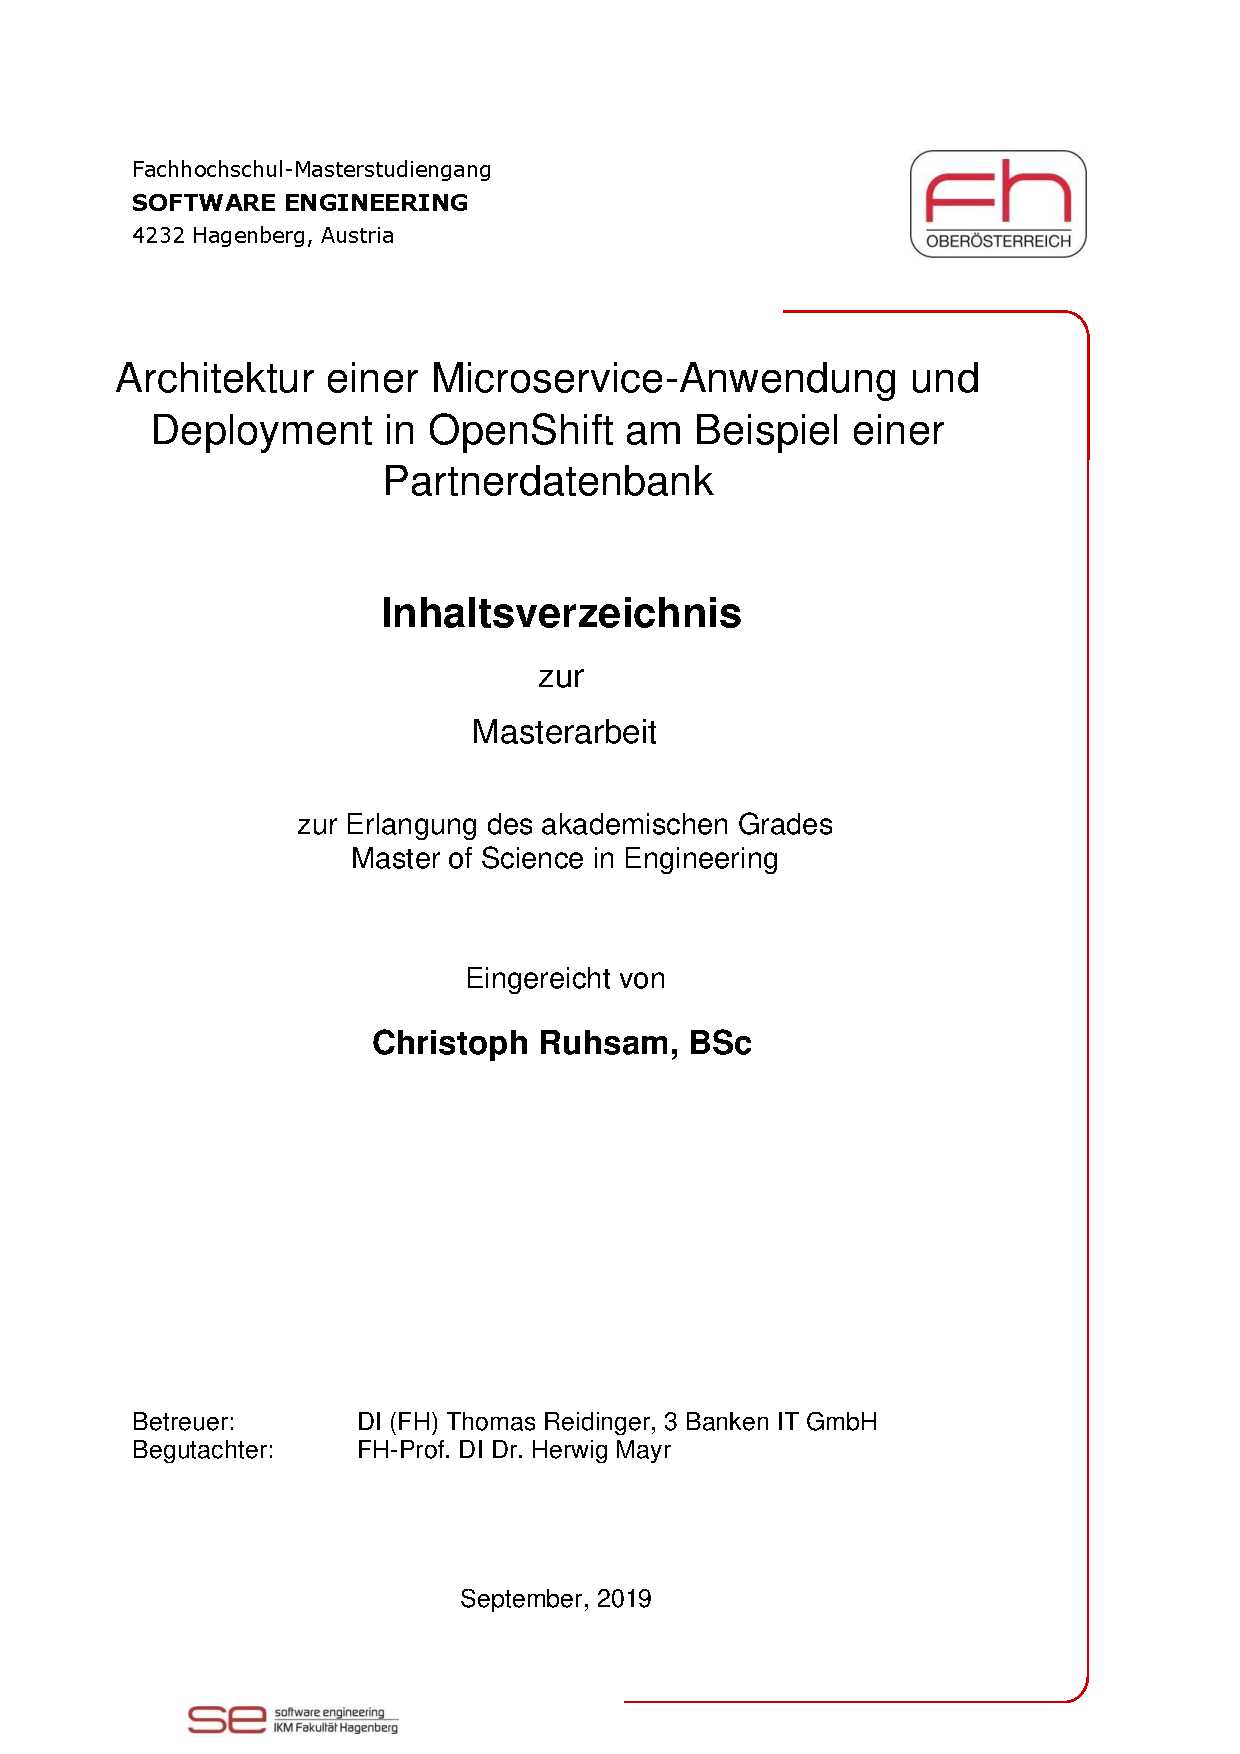
\includepdf{title.pdf}
%\maketitle
\tableofcontents

%\chapter{Preface}






 	% preface is optional
%\chapter{Abstract}
An Enterprise Service Bus (ESB) is a crucial part of an enterprise, which connects the enterprise to its partners, customers, and other branches. The appearance of containerization, cloud services, and the microservice architecture have provided new possibilities for implementing and running an ESB. But, an ESB is commonly used by large conservative enterprises, which don't adapt new technologies fast, and wait until a new technology has proven itself. Especially the cloud is something the industry denied to use for a long time, because of the fact, that the infrastructure and data are managed and maintained by external service providers. \\ 

These days, we live in the so called cloud age, whereby global enterprises like Red Hat or Amazon provide cloud services such as Platform as a Service (PaaS), which can scale with the business. Enterprises start to consider to move their ESB installations to the cloud to profit from the cloud service provided features. Moving an ESB to the cloud will be a long term process for an enterprise, because the established processes for development, running, and managing the ESB will have to change. \\

This thesis has the goal to give the reader an overview of the cloud related concepts and technologies such as, Infrastructure as Code (IaC) and Docker, which are the base for cloud services. The implemented ESB prototype,  is  available at \url{https://github.com/cchet-thesis-msc/prototype}, and shows how an ESB could be implemented on a PaaS platform. \\




%%%----------------------------------------------------------
\mainmatter          			% main part (arabic page numbers)
%%%----------------------------------------------------------

\chapter{Einleitung ... 5.5 Seiten}
\section{Motivation zur Architektur von Microservices ... 1.5 Seiten}
\section{Motivation zum Einsatz von Cloudtechnologien ... 1.5 Seiten}
\section{Zielsetzung der Implementierung der Partnerdatenbank ... 1 Seite}
\section{Ziel des Deployment der Partnerdatenbank in OpenShift ... 1 Seite}
\section{Leitfaden und Gliederung der Schrift ... 0.5 Seiten}

\chapter{Serviceorientierte Architektur und Microservices ... 12.5 Seiten}
\section{Definition und Abgrenzung ... 4 Seiten}
\section{Vergleich zu monolithischer Architektur ... 2 Seiten}
\section{Charakteristiken ... 3 Seiten}
\section{Varianten ... 1.5 Seiten}
\section{Vor- und Nachteile ... 2 Seiten}


\chapter{Containerisierung mit Docker ... 6 Seiten}
\section{Docker ... 4 Seiten}
\section{Notwendigkeit von Containerisierung ... 2 Seiten}


\chapter{OpenShift ... 10.5 Seiten}
\section{Beschreibung von OpenShift ... 2 Seiten}
\section{Komponenten von Kubernetes ... 3.5 Seiten}
\section{Die OpenShift-Umgebung ... 3 Seiten}
\section{Fabric8 ... 2 Seiten}

\chapter{Partnerdatenbank ... 14.5 Seiten}
\section{Grundaufbau und Ziel der Partnerdatenbank ... 2.5 Seiten}
\section{Backend-Beschreibung ... 4 Seiten}
\section{Beschreibung der einzelnen Services ... 4 Seiten}
\section{Frontend-Beschreibung ... 4 Seiten}

\chapter{Design der Partnerdatenbank ... 11 Seiten}
\section{Microservice-Architektur ... 3 Seiten}
\section{Beschreibung der verwendeten Microservice-Technologien ... 6 Seiten}
\section{Design in OpenShift .. 2 Seiten}


\chapter{Implementierung der Partnerdatenbank ... 17 Seiten}
\section{Microservice-Architektur ... 2 Seiten}
\section{Automatisierte Test-, Build- und Deployment-Pipelines mit Jenkins ... 3 Seiten}
\section{Fehlerbehandlung mit Microprofile ... 2 Seiten}
\section{REST-Schnittstellenbeschreibung mit Swagger ... 2 Seiten}
\section{Tracing mit Jaeger ... 1 Seite}
\section{Einsatz von Docker zur Containerisierung der Anwendung ... 1 Seite}
\section{Konfiguration und Deployment-Deskriptoren von OpenShift ... 4 Seiten}
\section{Deployment in OpenShift mit Fabric8 ... 2 Seiten}


\chapter{Evaluierung der Anwendung ... 5.5 Seiten}
\section{Evaluierung des Frontend ... 1.5 Seiten}
\section{Unittests ... 1 Seite}
\section{Integrationstests ... 1 Seite}
\section{Architekturevaluierung ... 2 Seiten}

\chapter{Zusammenfassung und Ausblick ... 2-3 Seiten}

\chapter{Quellenverzeichnis}



%%%----------------------------------------------------------
\end{document}
%%%----------------------------------------------------------